% This paper is part of the k2-paper project.
% Copyright 2015 Dan Foreman-Mackey (NYU) and the co-authors listed below.
%
%  RULES OF THE GAME
%
%  * 80 characters
%  * line breaks at the ends of sentences
%  * eqnarrys ONLY
%  * ``light curve'' not ``light-curve'' or ``lightcurve''
%  * Do not put in any comments that might get tweeted by @OverheardOnAph
%    (or maybe do put in a few....)
%  * that is all.
%

\documentclass[12pt,preprint]{aastex}

\pdfoutput=1

\usepackage{color,hyperref}
\definecolor{linkcolor}{rgb}{0,0,0.5}
\hypersetup{colorlinks=true,linkcolor=linkcolor,citecolor=linkcolor,
            filecolor=linkcolor,urlcolor=linkcolor}
\usepackage{url}
\usepackage{amssymb,amsmath}
\usepackage{subfigure}
\usepackage{booktabs}

\usepackage{natbib}
\bibliographystyle{apj}

\newcommand{\project}[1]{\textsl{#1}} % hogg say
\newcommand{\kepler}{\project{Kepler}}
\newcommand{\KT}{\project{K2}}
\newcommand{\tess}{\project{TESS}}
\newcommand{\jwst}{\project{JWST}}
\newcommand{\terra}{\project{TERRA}}
\newcommand{\pdc}{\project{PDC}}
\newcommand{\license}{MIT License}
\newcommand{\projectname}{\project{ketu}}

\newcommand{\paper}{\textsl{Article}}

\newcommand{\foreign}[1]{\emph{#1}}
\newcommand{\etal}{\foreign{et\,al.}}
\newcommand{\etc}{\foreign{etc.}}
\newcommand{\True}{\foreign{True}}
\newcommand{\Truth}{\foreign{Truth}}

\newcommand{\figref}[1]{\ref{fig:#1}}
\newcommand{\Fig}[1]{Figure~\figref{#1}}
\newcommand{\fig}[1]{\Fig{#1}}
\newcommand{\figlabel}[1]{\label{fig:#1}}
\newcommand{\Tab}[1]{Table~\ref{tab:#1}}
\newcommand{\tab}[1]{\Tab{#1}}
\newcommand{\tablabel}[1]{\label{tab:#1}}
\newcommand{\Eq}[1]{Equation~(\ref{eq:#1})}
\newcommand{\eq}[1]{\Eq{#1}}
\newcommand{\eqalt}[1]{Equation~\ref{eq:#1}}
\newcommand{\eqlabel}[1]{\label{eq:#1}}
\newcommand{\Sect}[1]{Section~\ref{sect:#1}}
\newcommand{\sect}[1]{\Sect{#1}}
\newcommand{\sectalt}[1]{\ref{sect:#1}}
\newcommand{\App}[1]{Appendix~\ref{sect:#1}}
\newcommand{\app}[1]{\App{#1}}
\newcommand{\sectlabel}[1]{\label{sect:#1}}

\newcommand{\BIC}{{\ensuremath{\mathrm{BIC}}}}
\newcommand{\TIC}{{\ensuremath{\mathrm{TIC}}}}
\newcommand{\T}{\ensuremath{\mathrm{T}}}
\newcommand{\dd}{\ensuremath{\,\mathrm{d}}}
\newcommand{\bvec}[1]{{\ensuremath{\boldsymbol{#1}}}}
\newcommand{\appropto}{\mathrel{\vcenter{
  \offinterlineskip\halign{\hfil$##$\cr
    \propto\cr\noalign{\kern2pt}\sim\cr\noalign{\kern-2pt}}}}}
\newcommand{\densityunit}{{\ensuremath{\mathrm{nat}^{-2}}}}

% TO DOS
\newcommand{\todo}[3]{{\color{#2} \emph{#1} TODO: #3}}
\newcommand{\dfmtodo}[1]{\todo{DFM}{red}{#1}}
\newcommand{\hoggtodo}[1]{\todo{HOGG}{blue}{#1}}

% Notation for this paper.
\newcommand{\flux}{{\ensuremath{f}}}
\newcommand{\ferr}{{\ensuremath{\sigma_\flux}}}
\newcommand{\attime}{{\ensuremath{t}}}
\newcommand{\basis}{{\bvec{A}}}
\newcommand{\weights}{{\bvec{w}}}

\newcommand{\period}{{\ensuremath{P}}}
\newcommand{\phase}{{\ensuremath{T^0}}}
\newcommand{\duration}{{\ensuremath{D}}}
\newcommand{\depth}{{\ensuremath{Z}}}
\newcommand{\transittime}{{\ensuremath{T}}}
\newcommand{\impact}{{\ensuremath{b}}}
\newcommand{\ecc}{{\ensuremath{e}}}
\newcommand{\pomega}{{\ensuremath{\omega}}}

\begin{document}

\title{%
    A systematic search for transiting planets in the \KT\ data
}

\newcommand{\nyu}{2}
\newcommand{\caltech}{3}
\newcommand{\cfa}{4}
\newcommand{\mpia}{5}
\newcommand{\cds}{6}
\newcommand{\princeton}{7}
\newcommand{\mpis}{8}
\author{%
    Daniel~Foreman-Mackey\altaffilmark{1,\nyu},
    Benjamin~T.~Montet\altaffilmark{\caltech,\cfa},
    David~W.~Hogg\altaffilmark{\nyu,\mpia,\cds},
    Timothy~D.~Morton\altaffilmark{\princeton},
    Dun~Wang\altaffilmark{\nyu},
    Bernhard~Sch\"olkopf\altaffilmark{\mpis},
    \etal
}
\altaffiltext{1}         {To whom correspondence should be addressed:
                          \url{danfm@nyu.edu}}
\altaffiltext{\nyu}      {Center for Cosmology and Particle Physics,
                          Department of Physics, New York University,
                          4 Washington Place, New York, NY, 10003, USA}
\altaffiltext{\caltech}  {California Institute of Technology, Pasadena, CA,
                          91125, USA}
\altaffiltext{\cfa}      {Harvard-Smithsonian Center for Astrophysics,
                          Cambridge, MA 02138, USA}
\altaffiltext{\mpia}     {Max-Planck-Institut f\"ur Astronomie,
                          K\"onigstuhl 17, D-69117 Heidelberg, Germany}
\altaffiltext{\cds}      {Center for Data Science,
                          New York University,
                          726 Broadway, 7th Floor, New York, NY, 10003, USA}
\altaffiltext{\princeton}{Department of Astrophysics, Princeton University,
                          Princeton, NJ, 08544, USA}
\altaffiltext{\mpis}     {Max Planck Institute for Intelligent Systems
                          Spemannstrasse 38, 72076 T\"ubingen, Germany}

\begin{abstract}

The photometry from the \KT\ extension of NASA's \kepler\ mission is
afflicted by systematic effects caused by the relative imprecision of the
telescope pointing and other spacecraft issues.
We present a method for searching these light curves for evidence of
exoplanets by simultaneously fitting for these systematics and the
transit signals of interest.
This method is more computationally expensive than standard search algorithms
but we demonstrate that it can be efficiently implemented and used to robustly
discover transit signals.
We apply this method to the full Campaign 1 dataset and report a list of XXX
planet candidates transiting YYY stars.
For all planet candidates, we present posterior distributions on the
properties of each system based strictly on the transit observables.
We also present a list of ZZZ candidate eclipsing binary systems.

\end{abstract}

\keywords{%
methods: data analysis
---
methods: statistical
---
catalogs
---
planetary systems
---
stars: statistics
}

\section{Introduction}

The \kepler\ Mission (cite something) has been incredibly successful at
finding transiting exoplanets in the light curves of stars (cite something).
The Mission has demonstrated that it is possible to routinely measure signals
in stellar light curves at the part-in-$10^5$ level.
Results from the primary mission include the detection of planet transits with
depths as small as 12 parts per million \citep{Barclay:2013}.

The noise floor for \kepler\ data is often quoted as 15 parts per million (ppm) per
six hours of observations \citep{Gilliland:2011}.
Although they generally do not interfere with searches for transiting
planets, larger systematic effects exist on different timescales.
One of the most serious of these is spacecraft pointing: If the detector
flat-field is not known with very high accuracy, then tiny changes to the relative
illumination of pixels caused by a star's motion in the focal plane will lead
to changes in the measured or inferred brightness of the star.

The great stability of the original \kepler\ Mission
came to an end with the failure of a critical reaction wheel.
The \KT\ Mission \citep{Howell:2014} is a follow-on to the primary Mission,
observing about a dozen fields near the ecliptic plane, each for
$\sim 75$ days at a time.
Because of the degraded spacecraft orientation systems, the new \KT\ data
exhibit far greater pointing variations---and substantially more
pointing-induced variations in photometry---than the original \kepler\ Mission data.
This makes good data-analysis techniques even more valuable.

Good photometry relies on either a near-perfect flat-field
and pointing model or else data-analysis techniques that are
insensitive to these instrument properties.
The flat-field for \kepler\ was measured on the ground before the launch of
the spacecraft, but is not nearly as accurate as required to make
pointing-insensitive photometric measurements at the relevant level of precision.
In principle direct inference of the flat-field might be possible;
however, because point sources are observed with relatively limited
spacecraft motion, and only a few percent of the data are actually stored and
downloaded to Earth, there isn't enough information in the data to derive or
infer a complete or accurate flat-field map.
Therefore, work on \KT\ is sensibly focused on building data-analysis
techniques that are pointing-insensitive.

Previous projects have developed methods to work with \KT\ data.
\citet{Vanderburg:2014} extract aperture photometry from the pixel data
and decorrelate with image centroid position, producing light curves for each
star that are ``corrected'' for the spacecraft motion.
These data have produced the first confirmed planet found with
\KT\ \citep{Vanderburg:2015}.
Both \citet{Aigrain:2015} and \citet{Crossfield:2015} use a Gaussian Process
model for the measured flux, with pointing measurements as the inputs, and
then ``de-trend'' using the mean prediction from that model.
Other data-driven approaches have been developed and applied to the \kepler\
data \citep[for example,][]{pdc1, pdc2, arc, dun} but they have yet to be
generalized to be applicable to \KT.

In all of these light-curve processing methodologies, the authors follow a
traditional procedure of ``correcting'' or ``de-trending'' the light curve to
remove systematic and stellar variability as a step that happens \emph{before}
the search for transiting planets.
Fit-and-subtract is dangerous:
Small signals, such as planet transits, can be
partially absorbed into the best-fit stellar variability or systematics
models, making each individual transit event appear shallower.
In other words, the traditional methods are prone to over-fitting.
Because over-fitting will in general reduce the amplitude of true exoplanet
signals, small planets that ought to appear just above any specific
signal-to-noise or depth threshold could be missed because of the de-trending.
This becomes especially important as the amplitude of the noise increases.

The alternative to this approach is to \emph{simultaneously fit} both the systematics
and the transit signals.
Simultaneous fitting can push the detection limits to lower signal-to-noise while
robustly accounting for uncertainties about the systematic trends.
In particular, it permits us to \emph{marginalize} over choices in the noise
model and propagate any uncertainties about the systematic effects
to our confidence in the detection.
This marginalization ensures that any conclusions we come to about the exoplanet
properties are conservative, given the freedom of the systematics model.

In this \paper\ we present a data-analysis technique for exoplanet search and
characterization that is insensitive to spacecraft-induced trends in the light
curves.
We assume that the trends in the observed light curves in each star due to
spacecraft motion are shared by other stars; the systematic effects are
modeled as sums of stars.
We reduce the dimensionality by running PCA on stellar light curves
to obtain the dominant modes.
The search for planets proceeds by modeling the data as a linear combination of
150 of these basis vectors and a transit model.
Our method builds on the ideas behind previous data-driven de-trending procedures
such as the \kepler\ pipeline pre-search data conditioning \citep[\pdc;][]{pdc1, pdc2},
but (because of our simultaneous fitting approach) we can use a
much more flexible systematics model without worrying about over-fitting.

The methods developed within this paper are highly relevant to both \KT\ and
the upcoming \tess\ mission \citep{Ricker:2014}.
\tess\ will feature pointing precision of $\sim 3$ arcseconds (cite), similar
to the level of pointing drift with \KT.
Moreover, the typical star will be only observed for one month at a time, and
the typical transit detection will be at a similar signal-to-noise ratio as
with \KT.

Catalogs of transiting planets found in the \KT\ data will be important to
better understand the physical properties, formation, and evolution of
planetary systems.
These planets, especially when they orbit bright or late-type
stars, will be useful targets for ground-based and space-based follow-up, both
for current facilities and those planned in the near future such as \jwst.
They will also deliver input data for next-generation population inferences
\citep{dfm}, especially for the population of planets around cool stars
\citep[for example,][]{dressing}.

The \paper\ is organized as follows.
In \sect{phot}, we describe our method of extracting aperture photometry from
the calibrated \KT\ postage stamp time series.
In \sect{model} (with details in \app{math}), we describe our data-driven
model for the systematic trends in the photometric light curves and our method
for fitting this model simultaneously with a transit signal.
In \sect{search}, we give the detailed procedure that we use for discovering
and vetting planet candidates.
To quantify the performance and detection efficiency of our pipeline, we test
(in \sect{perform}) the recovery and false alarm rate of synthetic transit
signals, spanning a large range of physical parameters, injected into real
\KT\ light curves.
Finally, in \sect{results}, we present a catalog of XXXX planet candidates
orbiting WWWW stars---and a supplementary list of YYYY eclipsing binary
candidates---in the publicly available \KT\ Campaign 1 dataset.


\section{Photometry and Eigen Light Curves}
\sectlabel{phot}

The starting point for analysis is the raw pixel data.
We download the full set of \dfmtodo{XXX} target pixel files for \KT's Campaign 1 from
MAST\footnote{\url{https://archive.stsci.edu/k2/}}.
We extract photometry using fixed circular apertures of varying sizes
centered on the predicted location of the target star based on the world
coordinate system.
\dfmtodo{In detail, the apertures are only approximately circular; in detail each pixel
gets a weight of unity if its center is in the circle, and zero otherwise.}
For each target, we performed the photometry in a set of
circular apertures ranging in radius from 0.5 to
5 pixels (in steps of 0.5 pixels) and---following
\citet{Vanderburg:2014}---chose the aperture size that resulted in the
smallest CDPP \citep{cdpp}
with a 6 hour window.\footnote{Note that although we chose a specific
aperture for each star, photometry for this aperture and every other
aperture size at which we easured is all available online at
\dfmtodo{some URL}.}

All previous methods for analyzing \KT\ data involve some sort of
``correction'' or ``de-trending'' step based on measurements of the pointing
of the spacecraft \citep{Vanderburg:2014, Aigrain:2015,
Crossfield:2015}.
In our analysis, we don't do any further preprocessing of the light curves
because, as we describe in the next section, we are going to simultaneously fit for the
trends and the transit signals that we are searching for in the raw
photometric light curves.

One key realization that is also exploited by the official \kepler\ pipeline
is that the systematic trends caused by pointing shifts and other instrumental
effects are shared---with different signs and weights---by all the stars on
the focal plane.
To capitalize on this, the \pdc\ component of the \kepler\ pipeline
removes any trends from the light curves that can be fit using a linear
combination of a small number of ``co-trending basis vectors''.
This basis of trends was found by running Principal Component Analysis (PCA)
on a large set of (filtered) light curves and extracting the top few ($\sim 4$)
components \citep{pdc1, pdc2}.
Similarly, we ran PCA on the full set of our own generated \KT\ Campaign~1 light curves to determine
a basis of representative trends but, unlike \pdc, we retain and use
a large number of these components ($150$).
For clarity, we will refer to our basis as a set of ``eigen light curves''
(ELCs) and the full set is made available online (\dfmtodo{SOMEURL}).
The top \dfmtodo{ten} ELCs for Campaign~1 are shown in \Fig{pca}.


\section{Joint transit \& variability model}
\sectlabel{model}

The key insight in our transit search method that sets it apart from the
other standard procedures is that no de-trending is necessary.
Instead, we can fit for the noise (or trends) and signal simultaneously.
This is theoretically appealing because it will be more sensitive to low
signal-to-noise transits.
The main reason for this is that the signal is not exactly orthogonal to the
systematics and any de-trending will over-fit; decreasing the amplitude of the
signal and distorting its shape.
In order to reduce this effect, most procedures use a very rigid model for
the trends.
For \KT, this has been implemented by asserting that the centroids contain
all of the information needed to describe the trends \citep{Vanderburg:2014,
Aigrain:2015, Crossfield:2015}.
In the \kepler\ pipeline, this is implemented by only allowing a small number
of PCA components to contribute to the fit in the \pdc\ procedure.
Instead, we will use a large number of ELCs---a very flexible model---and
use a physically motivated method to avoid over-fitting.

Physically, the motivation for our model---and the \pdc\ model---is that every
star on the detector should be affected by the same set of systematic effects.
These are caused by things like pointing jitter, temperature variations, and
other sources of PSF modulation and each one will be imprinted in the light
curves of many stars with varying amplitudes and signs as a result of the
varying flat field.
Therefore, while it is hard to write down a physical generative model for the
systematics, building a data-driven model might be possible.
This intuition is also exploited by other methods that model the systematics
using only empirical centroids \citep{Vanderburg:2014, Aigrain:2015,
Crossfield:2015} but our more flexible model should capture the systematic
effects more robustly.
For example, \Fig{corr} shows the application of our model---with 150
ELCs---to a light curve with no known transit signals and the precision is
excellent.
If, however, we were to apply this model blindly to a light curve with
transits, we would be at risk of over-fitting and decreasing the amplitude of
the signal.

To avoid over-fitting, in our pipeline we simultaneously fit for the transit
signal and the trends using a rigid model for the signal and a relatively
flexible model for the noise.
Specifically, we model the light curve as being generated by linear
combination of 150 ELCs and a ``box'' transit model at a specific period,
phase, and duration.
The mathematical details are given in \app{math} but in summary, since the
model is linear, we can analytically compute the likelihood
function---conditioned on a specific period, phase, and duration---for the
depth \emph{marginalized over the systematics model}.
The signal-to-noise of this depth measurement can then be used as a quality
of fit metric or candidate selection scalar.
This computation is expensive but, as described in the following sections, it
is possible to scale the method to a \KT-scale dataset.

It is worth noting that this model can be equivalently thought of as a
(computationally expensive) generalization of the ``Box Least Squares''
\citep[\project{BLS};][]{bls} method to a more sophisticated description of
the noise and systematics.
Therefore, any existing search pipeline based on \project{BLS} could, in
theory, use this model as a drop-in replacement, although some modifications
might be required for computational tractability.


\section{Search pipeline}
\sectlabel{search}

In principle, the search for transit signals simply requires evaluating the
model described above on a fine three-dimensional grid in period, phase, and
duration, and then detecting high significance peaks in that space.
In practice, this is computationally intractable for any grids of the
required size.
Instead, we can compute the values on this grid approximately, but at very
high precision, using a two-step procedure that is much more computationally
efficient.

Specifically, we must evaluate the likelihood function for the light curve of
star $n$ given a period \period, reference transit time \phase, and duration
\duration
\begin{eqnarray}\eqlabel{full-likelihood}
p(\{\flux\}_n\,|\,\period,\,\phase,\,\duration,\,\depth) \quad.
\end{eqnarray}
We make the simplifying assumption that each transit enters this quantity
independently because it is approximately satisfied for all but the shortest
periods and it leads to a huge computational advantage.
Under this assumption, this likelihood function can be rewritten as
\begin{eqnarray}\eqlabel{indtran}
p(\{\flux\}_n\,|\,\period,\,\phase,\,\duration,\,\depth) &=&
\prod_{m=1}^{M(\period,\,\phase)}
    p(\{\flux\}_n\,|\,\transittime_m(\period,\,\phase),\,\duration,\,
                    \depth)
\end{eqnarray}
where $\transittime_m(\period,\,\phase)$ is the time of the $m$-th
transit given the period $\period$ and reference time $\phase$.
\Eq{indtran} can be efficiently computed for many periods and phases if we
first compute a set of likelihood functions for single transits on a grid
in $\transittime_l$ and duration $\duration_k$
\begin{eqnarray}\eqlabel{singletransit}
\left \{ p(\{\flux\}_n\,|\,\transittime_l,\,\duration_k,\,\depth)
\right\}_{l=1,\,k=1}^{L,\,K} \quad.
\end{eqnarray}
Then, we can use these results as a look-up table to approximately evaluate
\eq{full-likelihood}.

In the remainder of this section, we give more details about each step of the
search procedure but in summary, it breaks into three main steps: linear
search, periodic search, and vetting.
In the {\bf linear search} step, we evaluate the likelihood function in
\eq{singletransit} on a two-dimensional grid, coarse in transit duration
$\duration_k$ and fine in transit time $\transittime_m$.
Then in the {\bf periodic search} step, we use this two-dimensional grid to
approximately evaluate the likelihood (\eqalt{indtran}) for a
three-dimensional grid of periodic signals.
Then, we run a peak detection algorithm on this grid that discards signals
with substantially varying transit depths.
These transit candidates are then passed along for machine and human {\bf
vetting}.


\paragraph{Linear search}

The linear search requires hypothesizing a set of transit signals on a
two-dimensional grid in transit time and duration.
For each point in the grid, we use the model described in \sect{model} to
evaluate \emph{the likelihood function} for the transit depth at that time
and duration.
Since the model is linear, the likelihood function for the depth (marginalized
over the model of the systematics) is a Gaussian with analytic amplitude $L$,
mean $\bar{\depth}$, and variance $\delta\bar{\depth}^2$ derived in
\app{math}.
Therefore in the linear search, we save these three numbers for a
two-dimensional grid in transit time $\transittime_l$ and duration
$\duration_k$.
The transit time grid spans the duration of Campaign 1 with half hour spacing
and we choose to only test three durations: 1.2, 2.4, and 4.8 hours.
\Fig{linear} shows the mean transit depth $\bar{\depth}$ as a function of
transit time \transittime\ for a light curve with an injected transit signal
with transits at the times indicated by the vertical green bars.

% The computational complexity of this step is $\mathcal{O}(M\,K^3)$ where $M$
% is the number of points in the grid and $K$ is the number of data points.


\paragraph{Periodic search}

In the period search step, we use the lookup table generated by the linear
search to compute the likelihood from \eq{indtran} on a three dimensional
grid in period \period, reference time \phase, and duration \duration.
At each point, we compute the likelihood of a model where the transit depth
varies between transits and the ``correct'' simpler model where the transit
depth is constant.
The variable depth likelihood is simply the product of amplitudes from the
initial search
\begin{eqnarray}
p_\mathrm{var}(\{\flux\}_n\,|\,\period,\,\phase,\,\duration) &=&
\prod_{m=1}^{M(\period,\,\phase)} L_m \quad,
\end{eqnarray}
and the constant depth model is
\begin{eqnarray}
p_\mathrm{const}(\{\flux\}_n\,|\,\period,\,\phase,\,\duration) &=&
\prod_{m=1}^{M(\period,\,\phase)}
    \frac{L_m}{\sqrt{2\,\pi\,{\delta\bar{\depth}_m}^2}}\,\exp \left(
        -\frac{[\depth - \bar{\depth}_m]^2}{2\,{\delta\bar{\depth}_m}^2}
    \right)
\end{eqnarray}
where the maximum likelihood depth is
\begin{eqnarray}\eqlabel{periodic-depth}
\depth &=& {\sigma_\depth}^2\,\sum_{m=1}^{M(\period,\,\phase)}
    \frac{\bar{\depth}_m}{{\delta\bar{\depth}_m}^2}
\end{eqnarray}
and the uncertainty on this depth is given by
\begin{eqnarray}\eqlabel{periodic-depth-uncert}
\frac{1}{{\sigma_\depth}^2} &=& \sum_{m=1}^{M(\period,\,\phase)}
    \frac{1}{{\delta\bar{\depth}_m}^2} \quad.
\end{eqnarray}
Note that this result is \emph{marginalized} over the parameters of the
systematics model.
Therefore, this estimate of the uncertainty on the depth takes any
uncertainty that we have about the systematics into account.

In general, the variable depth model will \emph{always} get a higher
likelihood because it is more flexible.
Therefore, to compare these two models, we use the Bayesian Information
Criterion (BIC).
The traditional definition of the BIC is
\begin{eqnarray}
-\frac{1}{2}\,\BIC_\cdot &=&
    \ln p_\cdot(\{\flux\}_n\,|\,\period,\,\phase,\,\duration)
    - \frac{J}{2} \ln N
\end{eqnarray}
where the likelihood function is maximized, $J$ is an estimate of the model
complexity and $N$ is the effective sample size.
To emphasize that $J$ and $N$ are tuning parameters of the method, we
redefine the BIC as the TIC
\begin{eqnarray}
\TIC_\cdot &=&
    \ln p_\cdot(\{\flux\}_n\,|\,\period,\,\phase,\,\duration) - \alpha
\end{eqnarray}
and we choose $\alpha$ heuristically.
For the K2 Campaign 1 dataset, we find that $\alpha \sim 1250$ leads to robust
recovery of injected signals while still being fairly insensitive to false
signals.

To limit memory consumption, in the periodic search, we actually profile (or
maximize) over \phase\ and \duration\ subject to the constraint that
$\TIC_\mathrm{const} > \TIC_\mathrm{var}$.
This results in a one-dimensional ``periodogram'' measuring the quality of
the fit as a function of period.
To choose the ``best'' candidate signal, we found that the best quantity to
select on was the signal-to-noise with which the depth was measured at a
given period, $\depth/\sigma_\depth$, computed using
Equations~(\ref{eq:periodic-depth}) and (\ref{eq:periodic-depth-uncert}).
Figure SOMEFIGURE shows the signal-to-noise of the depth measurement as a
function of period for SOMECANDIDATE.

After selecting the best candidate based on the signal-to-noise of the depth,
we mask out the sections of the linear search corresponding to these transits
and iterate the periodic search.
Under our assumption of independent transits, this is equivalent to removing
the sections of data that have a transit caused by the highest peak.
For the purposes of this \paper, we iterate the periodic search until we find
three peaks for each light curve.
This will necessarily miss the smallest and longest period planets in systems
with more than three transiting planets but given the precision---or lack
thereof---of the current method, we deemed this number sufficient.


\paragraph{Initial candidate list}

The periodic search procedure returned three signals per target so this gave
an initial list of ZZZZ candidates.
The vast majority of these signals are, of course, not induced by a
transiting planet.
Therefore to reduce the search space, we estimate the signal-to-noise of each
candidate by comparing the peak height to a robust estimate of variance in
\TIC\ values across period.
This is not the same criterion used to select the initial three peaks but we
found that at this stage, it produced a more complete and pure sample.
A cut in this quantity can reject most variable stars and low signal-to-noise
candidates that can't be reliably recovered from the data.
Figure SOMEFIGURE shows the distribution of signal-to-noise for a set of
injections and compares it to the distribution of false candidates that are
proposed by the pipeline.
To minimize contamination from false alarms but maximize our sensitivity, we
choose a threshold of 15.
We also find that the signals with periods $\lesssim 4$ days are very
contaminated by false alarms.
This might be because of the fact that our independence assumption
(SOMEEQUATION) breaks down at these short periods.
Therefore, we discard all signals with periods shorter than 4 days.
After these cuts, we're left with 741 candidates that we then examine by hand.
The full list of peaks and their relevant meta data is available online at
\dfmtodo{SOMEURL}.


\paragraph{Hand vetting}

After our initial cuts on the candidate list, the majority of signals are
still false alarms mostly due to variable stars or single outlying data
points.
It should be possible to construct a more robust machine vetting algorithm
that discards these samples without missing real transits (CITE SOME THINGS)
but for the purposes of this \paper, we simply inspect the light curve for
each of the YYYY candidates \emph{by hand} to discard signals that are not
convincing transits.
The results of this vetting can be seen online at SOMEURL.

This vetting resulted in a list of ZZZZ transiting candidates.
Many of these signals are due to astrophysical ``false positives'' like
eclipsing binaries or blending.
We address this effect in the following section and separate the list of
candidates into a list of astrophysical false positives and planet candidates.


\paragraph{Astrophysical false positives}

A major problem with any transit search is the potential confusion between
transiting planets and eclipsing binaries.
Ground-based surveys before \kepler\ often had a false-positive rate
of 30-40\%. (because of shit?)
In the primary \kepler\ mission, this number was significantly lower:
the false positive rate was only 5-10\% \citep{Morton:2011}.
Such improvement was enabled by the relatively small pixels, stable
pointing, and high precision of \kepler.
In \kepler\ data, false positives can be reliably separated from
planet candidates by looking for differences in the position of the
centroid of light during transit events with respect to the
out-of-transit data (e.g. citation), variations in the depth of
alternating transits (e.g. citation), and evidence for ellipsoidal
variations between transits (e.g. citation).

In \KT, the precision of these tests is lower and they must be applied with
care.
There are typically only a handful of transits, meaning differences between
``odd'' and ``even'' transits must be large to create a significant
difference.
Searching for ellipsoidal variations is hindered by the short time baseline
and the increased photometric uncertainty in \KT\ data.
Centroid variations are feasible in \KT\ but must be treated differently than
in the original \kepler\ mission where this effect was generally measured
using difference imaging (cite Howell).

To obtain an initial assessment of the astrophysical false positive rate in
our catalog of planet candidates, we test for significant centroid offsets
using the machinery that we have already established for modeling the
systematic trends in the data.
This is only the first word and a more complete characterization of our
catalog's reliability is forthcoming (Montet, Foreman-Mackey, \etal\ in prep).

To measure \emph{centroid offsets}, we start by empirically measuring the
pixel centroid time series for each candidate by modeling the pixels near the
peak as a two-dimensional quadratic and finding the maximum at each time.
This method has been shown to produce higher precision centroid measurements
than center-of-light estimates (@HOGG: is this true? Is there a citation? MJ
in prep?).
Figure SOMEFIGURE shows the measure $x$ and $y$ pixel coordinate traces for
SOMECANDIDATE.
Much like the photometry, this signal is dominated by the rigid body motion
of the spacecraft and we can, in fact, model it identically.
Previously (\eqalt{linear-model}), we modeled the light curve as a linear
combination of ELCs and a simple box transit model at a given period, phase,
and duration.
Under this model, the maximum likelihood depth can be computed analytically.
If we apply \emph{exactly the same model} to the centroid trace, the ``depth''
that we compute becomes the centroid motion in transit in units of pixels.
Since the motions won't necessarily point in a consistent direction across
transits, we treat each transit independently and report the average offset
amplitude weighted by the precision of each measurement.
To compute the significance of a centroid offset, we bootstrap the offset
amplitude for models at the same period and duration but randomly oriented
phases.
If the centroid measured for the candidate transit is substantially larger
than the random realizations, we label the candidate as a false positive.
In practice, the precision of the centroid measurements isn't sufficient to
robustly reject many candidates but of the list of 100 (RIGHT NUMBER), two
candidates---EPIC AAA and BBB---have offsets large enough that we remove them
from our final catalog.
Figure SOMEFIGURE shows the distribution of centroid offsets across the full
catalog.


\section{Performance}
\sectlabel{perform}

To test the performance and detection efficiency of our method, we conducted a
suite of XXXX injection and recovery tests, this is the result of 5 tests per
star.
For each test, we inject the signal from a realistic planetary system into the
raw aperture photometry of a random target and run the resulting light curve
through the full pipeline.
If the search returns a planet candidate---passing all of the same cuts as we
apply in the main search---with period and reference transit time within
HOWMANY days of the injected signal, we count that injection as recovered.
The detection efficiency of the search is approximately given by the fraction
of recovered injections as a function of the relevant parameters.

To generate the synthetic signals, we use the following procedure:
\begin{enumerate}

{\item Draw the number of transiting planets based on the observed
multiplicity distribution of KOIs (CITE).}

{\item Sample---from the distributions listed in
\tab{dist}---limb darkening parameters and, for each planet, an orbital
period, phase, radius ratio, impact parameter, eccentricity, and argument of
periapsis.}

{\item Based on the chosen physical parameters, simulate the light curve,
taking limb darkening and integration time into account \citep{ma,
kipping-int}, and multiply it into the raw aperture photometry.}

\end{enumerate}
We then process these light curves using exactly the pipeline that we use for
the light curves without injections.
Finally, we test for recovery after applying the cuts in signal-to-noise and
period.
We should, of course, also process the results of the injection tests by hand
to ensure that our measurements of detection efficiency aren't biased by this
step but, since we chose to limit our sample to very high signal-to-noise
candidates, it seems unlikely that our hand vetting removed any true transit
signals.
Any estimates of the false alarm rate will, however, be affected by this
negligence but we leave a treatment of this for future discussion.

\Fig{completeness} shows the fraction of recovered signals as a function of
the physical parameters of the injection and the magnitude of the star.
As expected, the shallower transits at longer periods are recovered less
robustly.
It is worth noting that this figure is a two-dimensional projection (or
marginalization) of a higher dimensional measurement.
For example, this completeness map is conditioned on our assumptions about
the eccentricity distribution of planets and it is marginalized over the
distribution of stellar parameters.
It is possible to relax this assumption and apply different distributions by
re-weighting the simulations used to generate this figure.
Therefore, alongside this \paper, we publish the full list of injection
simulations\footnote{SOMEURL} to be used for population inference (occurrence
rate measurements).
In \fig{completeness}, we also show the detection efficiency---marginalized
over the same range of periods---as a function of stellar magnitude in the
\kepler\ bandpass as reported in the EPIC.



\section{Results}
\sectlabel{results}

After running the 21XXX light curves through our full pipeline, we end up with
XXXX TCEs \dfmtodo{change this name} and after hand vetting by the two first
authors of this \paper, we are left with YYYY convincing transiting
candidates.
We choose to separate this list into two tables: planet candidates
(\tab{cand}) and eclipsing binary candidates (\tab{eb}).
For our purposes, we define an binary candidate as any system where we can
find a secondary eclipse by visual inspection but in most cases, the
secondary eclipse is also detected as a smaller transit signal at the same
period as the primary.
In this dataset, we discover ZZZ planet candidates around WWW stars.
Two of these were previously published \citep{Crossfield:2015} but, to our
knowledge, the remaining list is currently unpublished.
The third planet published by \citet{Crossfield:2015} is found as the third
signal for that target by our pipeline but it falls just below our
signal-to-noise cut so we left it out of the catalog for consistency.
This suggests that a less conservative cut in signal-to-noise and more
aggressive machine vetting could yield a much more complete catalog at smaller
radii and longer periods even with the existing dataset.

For the binaries, we simply list the period, phase, and depth determined by
the search algorithm but for the planet candidates, we perform a full physical
transit fit to the light curve.
To do this fit, we use Markov Chain Monte Carlo \citep[MCMC;][]{emcee} to
sample from the posterior probability for the stellar and planetary
parameters taking limb darkening and integration time into account.
In this fit, we continue to model the trends in the data as a linear
combination of 150 ELCs but, at this point, we combine this with a realistic
light curve model \citet{ma, kipping-ld}.
Even though we have no constraints on the stellar parameters, we also sample
over a large range in stellar mass and radius so that future measurements can
be applied by re-weighting the published samples.
In \tab{cand} we list the sample quantiles for the observable quantities and
the full chains are available electronically at \dfmtodo{some URL}.

SOMEFIGURE shows the distribution of radius ratios and periods of candidates
from our sample.


\section{Discussion}

We have searched the \KT\ Campaign~1 data set for exoplanet transit signals.
Our search is novel because it includes a very flexible systematics model,
which is fit simultaneously with the exoplanet signals of interest (and
marginalized out).
By this method, we find XXX new exoplanets, which we have vetted by ZZZ
method and characterized by probabilistic modeling.
The candidates are listed in \dfmtodo{some table} and
posterior distributions of planet candidate properties are available at
\dfmtodo{thisurl}.

The flexible systematics model we employ is a 150-parameter linear combination of PCA components
derived from the full set of 20,000 stellar lightcurves.
That is, it presumes that the systematics afflicting each star are shared in
some way across other stars.
It is our belief---although not a strict assumption of our model---that these
systematics are caused primarily by pointing drifts, or movements of the
pixels in the focal plane relative to the stars.
In principle, if the systematics \emph{are} dominated by pointing issues, the
systematics model could require only three parameters---three Euler
angles---not 150 amplitudes.
However, because (as the pointing drifts) each star sees it's own unique
local patch of flat-field variations, the mapping from pointing drifts to
brightness variations can be extremely non-linear.
Furthermore, because when the pointing is moving fast there is effectively
a smearing of the point-spread function, there are effects keyed to the
time derivative of the Euler angles as well.
The large number (150) of linear coefficients gives the linear model the
freedom to model complex non-linear behavior; we are trading off parsimony
in parameters with the enormous computational advantages of maintaining
linearity (and therefore also convexity).
The computational advantages of the linear model are three-fold:
Convexity obviates searching in parameter space for alternative modes;
linear least-squares optimization can be performed with simple linear algebra;
given Gaussian uncertainties and uninformative priors, marginalizations over
the linear parameters also reduces to pure linear algebra.

The goal of this \paper\ was to get exoplanet candidates out of the
\KT\ pixel-level data, it was \emph{not} to generate light curves.
That is, both the search phase and the characterization phase of the method
are approximations to computations of a likelihood function for the pixel
data telemetered down from the satellite.
We did not generate ``corrected'' or ``pre-search conditioned'' light-curves
at any stage; we simultaneously fit systematics and the signals of interest
to the raw data.
For this reason, there is no sense in which this method ever really
produces corrected light curves.
For us, a systematics-corrected light curve is not really a thing.

The posterior distributions we release are given in terms of observational
quantities (rather than physical quantities) and are specifically \emph{NOT}
marginalized over stellar properties.
In this work, we are agnostic about fundamental properties of the host stars.
The only assumptions we make are that the star targeted by the \KT\
team is truly the planet host, and that there is no dilution by other stars in
any aperture.
As a result, these posterior distributions reflect the maximum possible
uncertainty in parameters such as the planet radius, which depend sensitively
on properties of the host star.

To use these distributions to characterize the properties of specific systems,
one should weight our samples by inferred stellar properties...
Perhaps give a specific example here with some detailed discussion or math.

This is not the last time the \KT\ data will be searched!
There are many heuristic choices and short-cuts made in this search.
For example, the choice to work at 150 principal components is a choice
driven more by computational feasibility than any model selection or
utility optimization.
The systematics model is good for spacecraft-induced variability, but not
intrinsic stellar variability.
The systematics model has no concept of a physical model of the spacecraft or
the camera; that is, it makes little use of our prior information about how
\KT\ images are generated physically.
The search is performed with a box model and severe approximations are employed
to make it fast.
We don't consider planets (which must be abundant) on periods longer
than those that would leave two transits within the \KT\ Campaign~1
data set.

Most importantly, perhaps, the machine and hand vetting leave much to be desired...
list some deficiencies of the vetting.

The completeness and false-positive assessment could be vastly improved...
completeness estimates are not as extensive as desired;
there is essentially no estimate of the non-astrophysical false positive rate.
(There really is no proposal on the table anywhere for getting a false-positive
rate for the non-astrophysical FPs.)

We have not attempted to do any kind of populations analysis...
but presumably \KT\ data will rock this.  In what ways?

\acknowledgments
It is a pleasure to thank
Andrew Vanderburg (Harvard),
Ruth Angus (Oxford), Tom Barclay (Ames), \etal
for helpful contributions to the ideas and code presented here.
DFM, DWH, and DW were partially supported by the National Science Foundation
(grant IIS-1124794),
the National Aeronautics and Space Administration
(grant NNX12AI50G), and the Moore--Sloan Data Science Environment at NYU.
BTM was supported by a National Science Foundation Graduate Research
Fellowship (grant DGE‐1144469).

This research made use of the NASA \project{Astrophysics Data System} and the
NASA Exoplanet Archive.
The Archive is operated by the California Institute of Technology, under
contract with NASA under the Exoplanet Exploration Program.
This \paper\ includes data collected by the \kepler\ mission. Funding for the
\kepler\ mission is provided by the NASA Science Mission directorate.
These data were obtained from the Mikulski Archive for Space Telescopes
(MAST).
STScI is operated by the Association of Universities for Research in
Astronomy, Inc., under NASA contract NAS5-26555.
Support for MAST is provided by the NASA Office of Space Science via grant
NNX13AC07G and by other grants and contracts.

{\it Facilities:} \facility{Kepler}

\appendix

\section{Mathematical model}
\sectlabel{math}

Formally, this can be written for the light curve of the $k$-th star as
\begin{eqnarray}\eqlabel{linear-model}
\bvec{f}_k &=& \bvec{A}\,\bvec{w}_k + \mathrm{noise}
\end{eqnarray}
where
\begin{eqnarray}
\bvec{f}_k &=& \left (\begin{array}{cccc}
    f_{k,1} & f_{k,2} & \cdots & f_{k,N}
\end{array}\right )^\T
\end{eqnarray}
is the list aperture fluxes for star $k$ observed at $N$ times
\begin{eqnarray}
\bvec{t} &=& \left (\begin{array}{cccc}
    t_{1} & t_{2} & \cdots & t_{N}
\end{array}\right )^\T \quad.
\end{eqnarray}
In \eq{linear-model}, the design matrix is given by
\begin{eqnarray}
\bvec{A} &=& \left (\begin{array}{cccccc}
    x_{1,1} & x_{2,1} & \cdots & x_{J,1} & 1 & m_\bvec{\theta}(t_1) \\
    x_{1,2} & x_{2,2} & \cdots & x_{J,2} & 1 & m_\bvec{\theta}(t_2) \\
    && \vdots &&&\\
    x_{1,N} & x_{2,N} & \cdots & x_{J,N} & 1 & m_\bvec{\theta}(t_N)
\end{array}\right )
\end{eqnarray}
where the $x_{j,n}$ are the basis ELCs---with the index $j$ running over
components and the index $n$ running over time---and $m_\bvec{\theta}(t)$ is
the transit model
\begin{eqnarray}
m_\bvec{\theta}(t) &=& \left\{\begin{array}{cl}
-1 & \mathrm{if\,}t\,\mathrm{in\,transit} \\
0 & \mathrm{otherwise}
\end{array}\right.
\end{eqnarray}
parameterized by a period, phase, and transit duration (these parameters are
denoted by \bvec{\theta}).

Assuming that the uncertainties on $\bvec{f}_k$ are Gaussian and constant,
the maximum likelihood solution for \bvec{w} is
\begin{eqnarray}
{\bvec{w}_k}^* &\gets& \left( \bvec{A}^\T\,\bvec{A} \right)^{-1}\,
                       \bvec{A}^\T\,\bvec{f}_k
\end{eqnarray}
and the marginalized likelihood function for the transit depth is a Gaussian
with the mean given by the last element of ${\bvec{w}_k}^*$ and the variance
given by the lower-right element of the matrix
\begin{eqnarray}
{\bvec{\delta w}_k}^2 &\gets& {\sigma_k}^2 \,
            \left( \bvec{A}^\T\,\bvec{A} \right)^{-1}
\end{eqnarray}
where $\sigma_k$ is the uncertainty on $\bvec{f}_k$.
The amplitude of this Gaussian is given by
\begin{eqnarray}\eqlabel{depth-likelihood}
\mathcal{L}_k &=& \frac{1}{(2\,\pi\,{\sigma_k}^2)^{N/2}}\,\exp\left(
-\frac{1}{2\,{\sigma_k}^2}\,
\left| \bvec{f}_k - \bvec{A}\,{\bvec{w}_k}^* \right|^2
\right)
\end{eqnarray}
evaluated at the maximum likelihood value ${\bvec{w}_k}^*$.

Remember that the likelihood defined in \eq{depth-likelihood} is a function of
the parameters \bvec{\theta} (the period, phase, and duration of the planet).
In principle, this means that a transit search can proceed by building a dense
3D grid of \bvec{\theta} values and evaluating the likelihood of the data
$\mathcal{L}_k$ using \eq{depth-likelihood} at each point in the grid.

\clearpage
\bibliography{k2}
\clearpage


\begin{figure}[p]
\begin{center}
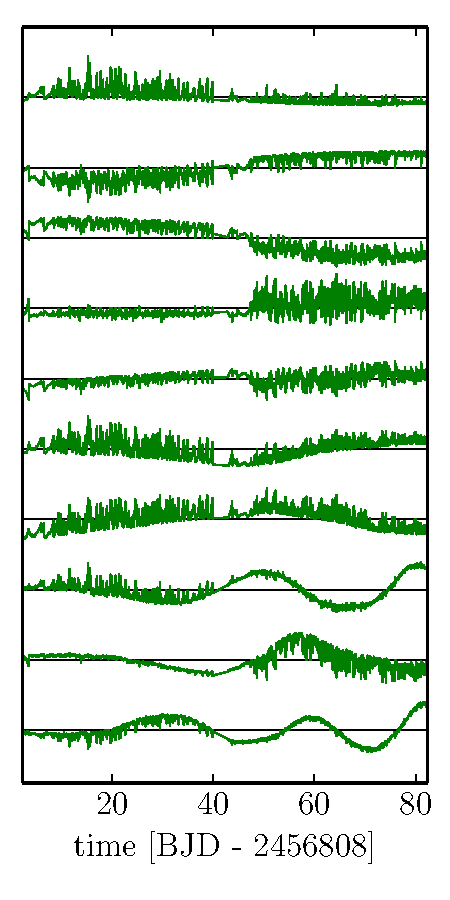
\includegraphics{figures/pca.pdf}
\end{center}
\caption{%
The top 10 eigen light curves (ELCs) generated by running principal component
analysis on all the aperture photometry from Campaign 1.
\figlabel{pca}}
\end{figure}

\begin{figure}[p]
\begin{center}
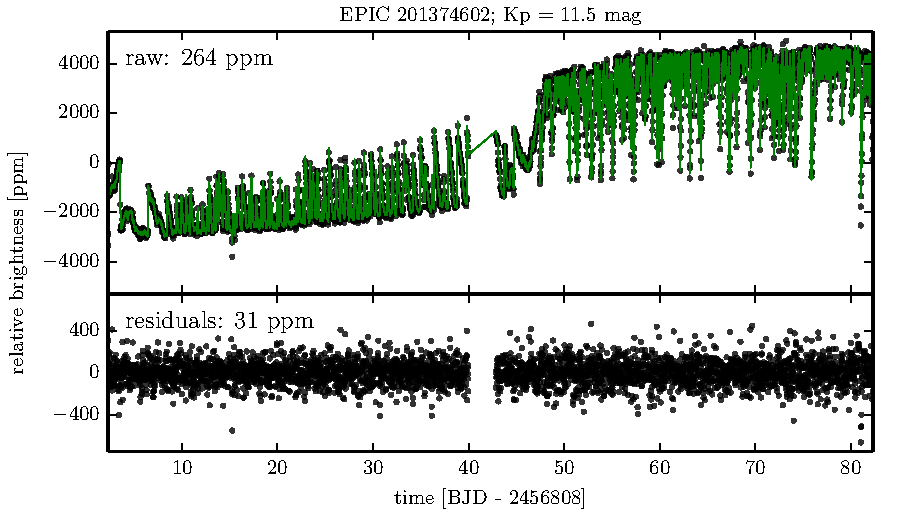
\includegraphics{figures/corr.pdf}
\end{center}
\caption{%
A demonstration of the ELC fit to the aperture photometry for EPIC 201374602.
\emph{Top:} The black points show the aperture photometry and the green line
is the maximum likelihood linear combination of ELCs.
The estimated 6-hour precision of the raw photometry is 264 ppm.
\emph{Bottom:} The points show the residuals of the data away from the ELC
prediction.
The 6-hour precision of this light curve is 31 ppm.
\figlabel{corr}}
\end{figure}

\begin{figure}[p]
\begin{center}
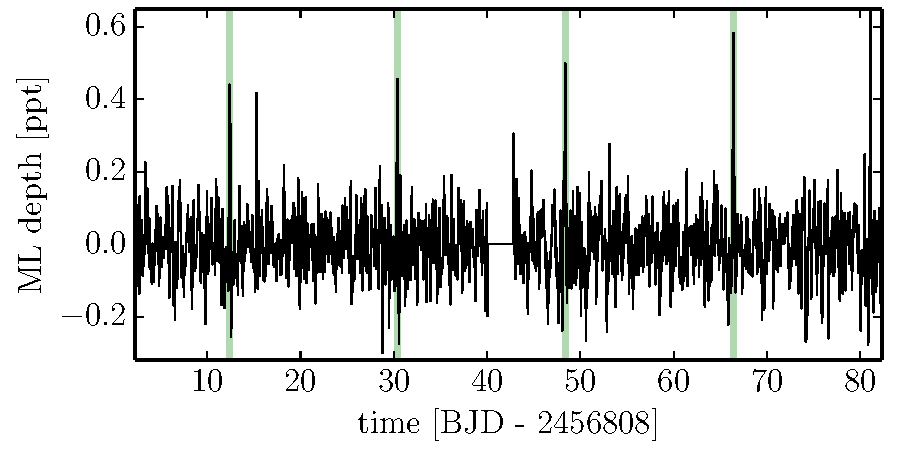
\includegraphics{figures/linear.pdf}
\end{center}
\caption{%
The estimated transit depth as a function of transit time as computed in a
linear search.
This light curve has an injected signal with transits at the times indicated
with green vertical lines.
\figlabel{linear}}
\end{figure}

\begin{figure}[p]
\begin{center}
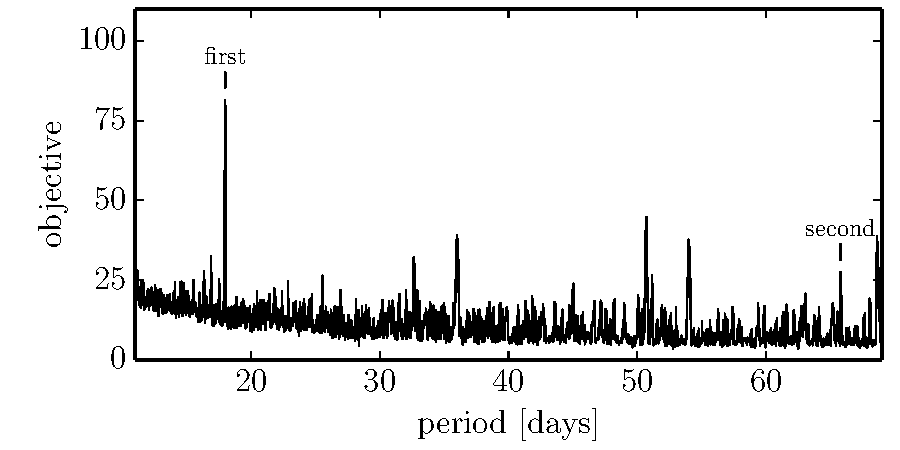
\includegraphics{figures/periodic.pdf}
\end{center}
\caption{%
The periodogram for the same signal as in \fig{linear}.
This plot was generated by the periodic search procedure.
The true period is indicated by the vertical green line.
\figlabel{periodic}}
\end{figure}

\begin{figure}[p]
\begin{center}
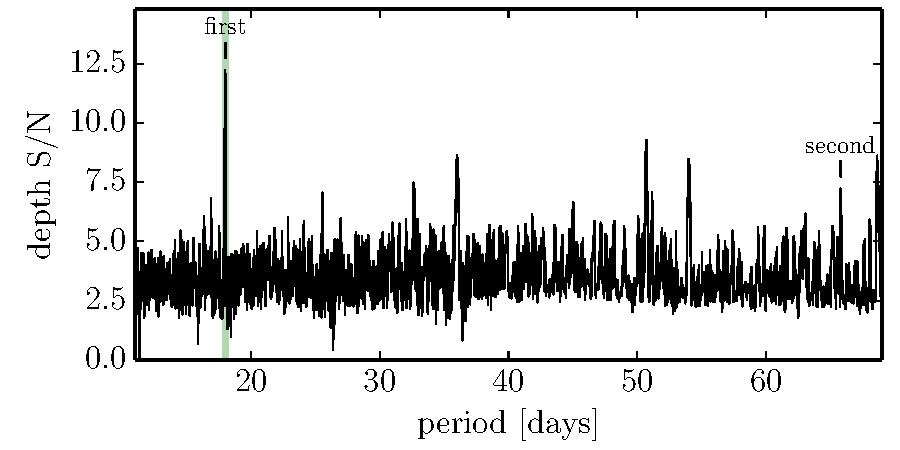
\includegraphics{figures/depth_s2n.pdf}
\end{center}
\caption{%
The signal-to-noise of the transit depth as a function of period for the same
signal as in \fig{periodic}.
The correct injected period is indicated by the vertical green line.
\figlabel{depth-s2n}}
\end{figure}

\begin{figure}[p]
\begin{center}
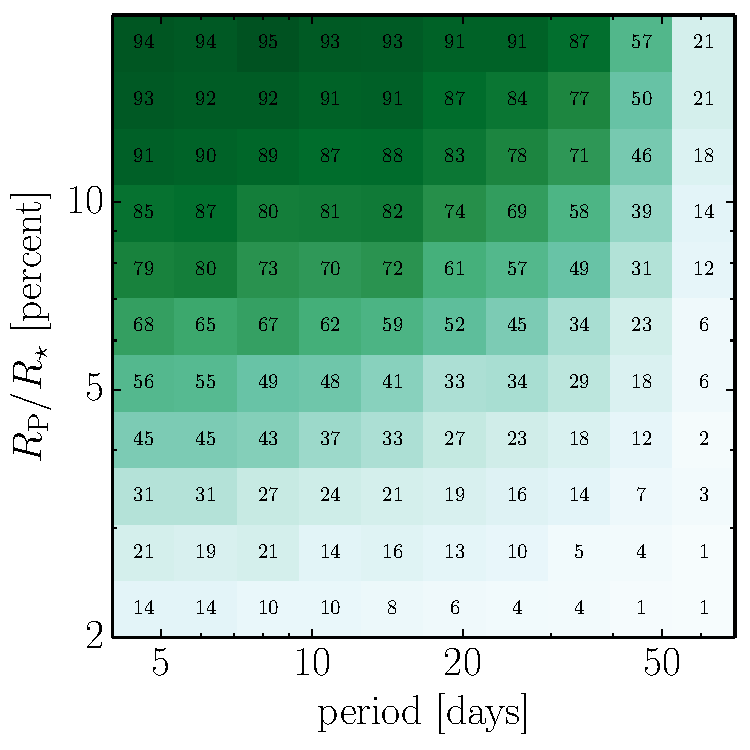
\includegraphics[width=\textwidth]{figures/completeness.pdf}
\end{center}
\caption{%
\figlabel{completeness}}
\end{figure}

\clearpage

\begin{table}[p]
\begin{center}
\begin{tabular}{lcc}
\toprule
Parameter & Units & Distribution \\
\midrule

limb darkening parameters $q_1$ and $q_2$ & --- & $q \sim U(0,\,1)$ \\
orbital period \period & days & $\ln \period \sim U(\ln 0.5,\,\ln 70)$ \\
reference transit time \phase & days & $\phase \sim U(0,\,\period)$ \\
radius ratio $R_P/R_\star$ & --- & $\ln R_P/R_\star \sim U(\ln 0.02,\,\ln 0.2)$ \\
impact parameter \impact & --- & $\impact \sim U(0,\,1)$ \\
eccentricity \ecc & --- & $\ecc \sim \mathrm{Beta}(0.867,\,3.03)$ \\
argument of periapsis \pomega & --- & $\pomega \sim U(-\pi,\,\pi)$ \\

\bottomrule
\end{tabular}
\end{center}
\caption{%
The distribution of physical parameters for the injected signals.
The eccentricity distribution is based on \citet{kipping-ecc} and the
limb darkening parameterization is given by \citet{kipping-ld}.
\tablabel{dist}}
\end{table}

\begin{table}[p]
\begin{center}
\small
\begin{tabular}{cccc}
\toprule
EPIC &  \period\ [days] & $t_0$ [BJD-2456808] & $R_\mathrm{P} / R_\star$ \\
\midrule
201208431 & $10.0040_{-0.0016}^{+0.0018}$ & $7.5216_{-0.0090}^{+0.0098}$ & $0.0349_{-0.0026}^{+0.0034}$ \\
201257461 & $50.2677_{-0.0074}^{+0.0083}$ & $20.3735_{-0.0098}^{+0.0147}$ & $0.0334_{-0.0017}^{+0.0054}$ \\
201280613 & $40.1205_{-0.0074}^{+0.0066}$ & $38.7724_{-0.0075}^{+0.0052}$ & $0.1508_{-0.0182}^{+0.0569}$ \\
201295312 & $5.6562_{-0.0007}^{+0.0007}$ & $3.7228_{-0.0091}^{+0.0086}$ & $0.0175_{-0.0009}^{+0.0020}$ \\
201338508 & $10.9328_{-0.0021}^{+0.0022}$ & $6.5967_{-0.0081}^{+0.0088}$ & $0.0339_{-0.0030}^{+0.0025}$ \\
201338508 & $5.7350_{-0.0006}^{+0.0006}$ & $0.8626_{-0.0055}^{+0.0054}$ & $0.0331_{-0.0023}^{+0.0025}$ \\
201367065 & $10.0542_{-0.0004}^{+0.0004}$ & $5.4186_{-0.0018}^{+0.0018}$ & $0.0354_{-0.0011}^{+0.0022}$ \\
201367065 & $24.6470_{-0.0016}^{+0.0014}$ & $4.2769_{-0.0029}^{+0.0030}$ & $0.0272_{-0.0013}^{+0.0016}$ \\
201384232 & $30.9375_{-0.0052}^{+0.0029}$ & $19.5035_{-0.0039}^{+0.0053}$ & $0.0260_{-0.0011}^{+0.0011}$ \\
201393098 & $28.6793_{-0.0116}^{+0.0105}$ & $16.6212_{-0.0177}^{+0.0305}$ & $0.0231_{-0.0020}^{+0.0028}$ \\
201403446 & $19.1535_{-0.0050}^{+0.0050}$ & $7.3437_{-0.0143}^{+0.0116}$ & $0.0154_{-0.0013}^{+0.0014}$ \\
201445392 & $10.3527_{-0.0011}^{+0.0011}$ & $5.6110_{-0.0051}^{+0.0047}$ & $0.0349_{-0.0025}^{+0.0045}$ \\
201445392 & $5.0644_{-0.0006}^{+0.0006}$ & $5.0690_{-0.0064}^{+0.0059}$ & $0.0274_{-0.0020}^{+0.0025}$ \\
201465501 & $18.4488_{-0.0015}^{+0.0015}$ & $14.6719_{-0.0032}^{+0.0035}$ & $0.0531_{-0.0039}^{+0.0061}$ \\
201505350 & $11.9069_{-0.0004}^{+0.0005}$ & $9.2764_{-0.0015}^{+0.0013}$ & $0.0446_{-0.0006}^{+0.0009}$ \\
201505350 & $7.9193_{-0.0001}^{+0.0001}$ & $5.3840_{-0.0008}^{+0.0006}$ & $0.0747_{-0.0013}^{+0.0016}$ \\
201546283 & $6.7713_{-0.0001}^{+0.0001}$ & $4.8453_{-0.0011}^{+0.0012}$ & $0.0481_{-0.0012}^{+0.0020}$ \\
201549860 & $5.6083_{-0.0006}^{+0.0005}$ & $4.1195_{-0.0047}^{+0.0045}$ & $0.0283_{-0.0023}^{+0.0041}$ \\
201555883 & $5.7966_{-0.0002}^{+0.0002}$ & $5.3173_{-0.0050}^{+0.0027}$ & $0.0604_{-0.0032}^{+0.0068}$ \\
201565013 & $8.6381_{-0.0002}^{+0.0003}$ & $3.4283_{-0.0015}^{+0.0016}$ & $0.1538_{-0.0243}^{+0.0355}$ \\
201569483 & $5.7969_{-0.0000}^{+0.0000}$ & $5.3130_{-0.0003}^{+0.0002}$ & $0.3587_{-0.0334}^{+0.0379}$ \\
201577035 & $19.3062_{-0.0013}^{+0.0013}$ & $11.5790_{-0.0027}^{+0.0025}$ & $0.0380_{-0.0012}^{+0.0023}$ \\
201593422 & $43.8753_{-0.0318}^{+0.0717}$ & $8.0383_{-0.0790}^{+0.0244}$ & $0.1366_{-0.0264}^{+0.0786}$ \\
201596316 & $39.8415_{-0.0155}^{+0.0136}$ & $21.8572_{-0.0101}^{+0.0120}$ & $0.0267_{-0.0022}^{+0.0034}$ \\
201613023 & $8.2818_{-0.0007}^{+0.0006}$ & $7.3752_{-0.0052}^{+0.0055}$ & $0.0205_{-0.0008}^{+0.0012}$ \\
201617985 & $7.2823_{-0.0008}^{+0.0007}$ & $4.6337_{-0.0050}^{+0.0050}$ & $0.0333_{-0.0032}^{+0.0072}$ \\
201629650 & $40.0492_{-0.0259}^{+0.0186}$ & $4.5363_{-0.0172}^{+0.0202}$ & $0.0241_{-0.0020}^{+0.0025}$ \\
201635569 & $8.3681_{-0.0002}^{+0.0002}$ & $3.4514_{-0.0014}^{+0.0015}$ & $0.0991_{-0.0078}^{+0.0120}$ \\
201649426 & $27.7704_{-0.0001}^{+0.0001}$ & $13.3476_{-0.0002}^{+0.0001}$ & $0.4365_{-0.0583}^{+0.0777}$ \\
201702477 & $40.7365_{-0.0025}^{+0.0026}$ & $3.5451_{-0.0025}^{+0.0026}$ & $0.0808_{-0.0114}^{+0.0043}$ \\
201736247 & $11.8106_{-0.0019}^{+0.0016}$ & $3.8483_{-0.0071}^{+0.0093}$ & $0.0347_{-0.0024}^{+0.0030}$ \\
201754305 & $19.0726_{-0.0049}^{+0.0048}$ & $1.4893_{-0.0133}^{+0.0128}$ & $0.0297_{-0.0030}^{+0.0042}$ \\
201754305 & $7.6202_{-0.0011}^{+0.0012}$ & $3.6813_{-0.0057}^{+0.0061}$ & $0.0281_{-0.0026}^{+0.0034}$ \\
201779067 & $27.2429_{-0.0001}^{+0.0001}$ & $12.2599_{-0.0003}^{+0.0002}$ & $0.2535_{-0.0259}^{+0.0369}$ \\
201828749 & $33.5093_{-0.0018}^{+0.0023}$ & $5.1554_{-0.0032}^{+0.0037}$ & $0.0267_{-0.0020}^{+0.0021}$ \\
201855371 & $17.9715_{-0.0017}^{+0.0015}$ & $9.9412_{-0.0038}^{+0.0033}$ & $0.0311_{-0.0017}^{+0.0030}$ \\
201912552 & $32.9410_{-0.0032}^{+0.0039}$ & $28.1834_{-0.0105}^{+0.0057}$ & $0.0513_{-0.0056}^{+0.0035}$ \\
201929294 & $5.0084_{-0.0001}^{+0.0001}$ & $4.5703_{-0.0012}^{+0.0022}$ & $0.1163_{-0.0014}^{+0.0011}$ \\
\bottomrule
\end{tabular}

\end{center}
\caption{%
Candidates
\tablabel{cand}}
\end{table}

\begin{table}[p]
\begin{center}
\begin{tabular}{cccc}
\toprule
EPIC & \period\ [days] & $t_0$ [BJD-2456808] & depth [ppt] \\
\midrule
201161715 & 59.81$^\mathrm{a}$ & 32.36 &  68.04 \\
201158453 &  7.07 &  5.46 &  72.75 \\
201160323 & 22.27 &  3.48 & 251.54 \\
201173390 & 17.00 &  8.40 &  31.34 \\
201333466 & 11.00 &  6.84 &  45.39 \\
201359834 & 40.11 & 30.66 &  11.92 \\
201368515 & 14.92 & 12.60 & 111.52 \\
201379113 & 42.41 & 14.24 & 210.28 \\
201382417 &  5.19 &  3.06 &  38.56 \\
201390608 &  9.81 &  4.58 &  82.85 \\
201408204 &  8.47 &  2.02 & 195.42 \\
201464977 & 15.89 &  1.50 &   8.18 \\
201530296 & 10.33 &  6.28 & 198.24 \\
201638314 &  5.43 &  4.30 &  49.66 \\
201648133 & 35.01 &  5.80 & 191.93 \\
201723461 & 22.73 & 22.14 & 262.30 \\
201763507 & 11.23 &  6.58 &   1.85 \\
201790675 & 33.83 & 29.10 & 352.43 \\
\bottomrule
\end{tabular}

\end{center}
\caption{%
Probable binaries.
\tablabel{eb}}
\end{table}

\end{document}
